\documentclass[frenchb, oneside, headings=normal]{scrartcl}

\usepackage[utf8x]{inputenc}
\usepackage[T1]{fontenc}
\usepackage{lmodern}

\usepackage{ifthen}
\usepackage{url}


\usepackage{multirow}

% Color
% cfr http://en.wikibooks.org/wiki/LaTeX/Colors
\usepackage{color}
\usepackage[usenames,dvipsnames,svgnames,table]{xcolor}
\definecolor{dkgreen}{rgb}{0.25,0.7,0.35}
\definecolor{dkred}{rgb}{0.7,0,0}

\newcommand{\matlab}{\textsc{Matlab}}

% Math symbols
\usepackage{amsmath}
\usepackage{amssymb}
\usepackage{amsthm}
\DeclareMathOperator*{\argmin}{arg\,min}
\DeclareMathOperator*{\argmax}{arg\,max}


% Sets
\newcommand{\Z}{\mathbb{Z}}
\newcommand{\R}{\mathbb{R}}
\newcommand{\Rn}{\R^n}
\newcommand{\Rnn}{\R^{n \times n}}
\newcommand{\C}{\mathbb{C}}
\newcommand{\K}{\mathbb{K}}
\newcommand{\Kn}{\K^n}
\newcommand{\Knn}{\K^{n \times n}}

% Unit vectors
\usepackage{esint}
\usepackage{esvect}
\newcommand{\kmath}{k}
\newcommand{\xunit}{\hat{\imath}}
\newcommand{\yunit}{\hat{\jmath}}
\newcommand{\zunit}{\hat{\kmath}}
\newcommand{\uunit}{\hat{\umath}}

% rot & div & grad & lap
\DeclareMathOperator{\newdiv}{div}
\newcommand{\divn}[1]{\nabla \cdot #1}
\newcommand{\rotn}[1]{\nabla \times #1}
\newcommand{\grad}[1]{\nabla #1}
\newcommand{\gradn}[1]{\nabla #1}
\newcommand{\lap}[1]{\nabla^2 #1}


% Elec
\newcommand{\B}{\vec B}
\newcommand{\E}{\vec E}
\newcommand{\EMF}{\mathcal{E}}
\newcommand{\perm}{\varepsilon} % permittivity

\newcommand{\bigoh}{\mathcal{O}}
\newcommand\eqdef{\triangleq}

\DeclareMathOperator{\newdiff}{d} % use \dif instead
\newcommand{\dif}{\newdiff\!}
\newcommand{\fpart}[2]{\frac{\partial #1}{\partial #2}}
\newcommand{\ffpart}[2]{\frac{\partial^2 #1}{\partial #2^2}}
\newcommand{\fdpart}[3]{\frac{\partial^2 #1}{\partial #2\partial #3}}
\newcommand{\fdif}[2]{\frac{\dif #1}{\dif #2}}
\newcommand{\ffdif}[2]{\frac{\dif^2 #1}{\dif #2^2}}
\newcommand{\constant}{\ensuremath{\mathrm{cst}}}

\usepackage{siunitx}

\usepackage{tikz}

\usepackage{pgfplots}
\usepackage{lmodern}
\usepackage{microtype}
\usepackage{xspace}

\usepackage{babel}
% Listing
% always put it after babel
% http://tex.stackexchange.com/questions/100717/code-in-lstlisting-breaks-document-compile-error
\usepackage{listings}

\definecolor{mygreen}{rgb}{0,0.6,0}
\definecolor{mygray}{rgb}{0.5,0.5,0.5}
\definecolor{mymauve}{rgb}{0.58,0,0.82}
\lstset{ %
  language=Matlab,
  backgroundcolor=\color{white},   % choose the background color; you must add \usepackage{color} or \usepackage{xcolor}
  basicstyle=\footnotesize,        % the size of the fonts that are used for the code
  breakatwhitespace=false,         % sets if automatic breaks should only happen at whitespace
  breaklines=true,                 % sets automatic line breaking
  captionpos=b,                    % sets the caption-position to bottom
  commentstyle=\color{mygreen},    % comment style
  deletekeywords={...},            % if you want to delete keywords from the given language
  escapeinside={\%*}{*)},          % if you want to add LaTeX within your code
  extendedchars=true,              % lets you use non-ASCII characters; for 8-bits encodings only, does not work with UTF-8
  frame=single,	                   % adds a frame around the code
  keepspaces=true,                 % keeps spaces in text, useful for keeping indentation of code (possibly needs columns=flexible)
  keywordstyle=\color{blue},       % keyword style
  otherkeywords={*,...},           % if you want to add more keywords to the set
  numbers=none,                    % where to put the line-numbers; possible values are (none, left, right)
  numbersep=5pt,                   % how far the line-numbers are from the code
  numberstyle=\tiny\color{mygray}, % the style that is used for the line-numbers
  rulecolor=\color{black},         % if not set, the frame-color may be changed on line-breaks within not-black text (e.g. comments (green here))
  showspaces=false,                % show spaces everywhere adding particular underscores; it overrides 'showstringspaces'
  showstringspaces=false,          % underline spaces within strings only
  showtabs=false,                  % show tabs within strings adding particular underscores
  stepnumber=2,                    % the step between two line-numbers. If it's 1, each line will be numbered
  stringstyle=\color{mymauve},     % string literal style
  tabsize=2,	                   % sets default tabsize to 2 spaces
  title=\lstname                   % show the filename of files included with \lstinputlisting; also try caption instead of title
}

\KOMAoptions{DIV=last}

\usepackage[top = 2.5 cm, bottom = 3 cm, left = 2.5 cm, right = 2.5 cm]{geometry}
\usepackage{caption}


\usepackage{epstopdf}
\begin{document}

\title{Projet ELEC Master 1 - Labo 3}
\subtitle{Groupe 4}
\author{Deprez Damien \and Bilal Ouachalih }
\date{10 octobre 2016}
\maketitle

The aim of this lab is to solve the problem of symbol timing recovery also known as symbol synchronization.

\section{Pre-Lab}

First, the model for the wireless communication channel is the following

\begin{equation}
z(t)=\alpha\exp^{j\phi} x(t-\tau_{d})+v(t)
\label{equ1}
\end{equation}

with $\alpha$ which is the attenuation, $\phi$ is the phase shift and $tau_d$ is the delay.

\subsection{Show that in the absence of noise, $\alpha$ and $\phi$ in the equation \ref{equ1} do not have any impact on the maximum output energy solution.} 

If we compute the expression of output energy, we can write it like this

\begin{equation}
J(\tau)=\mathbb{E}\|y(nT+\tau)|^2
\label{equ2}
\end{equation}

with $y[n]=\sqrt{E_x}\alpha\exp^{j\phi}s[n]+v[m]$.

As we can see, if we maximize the equation \ref{equ2}, we take the module squarred of y[n]. Like the module of $\alpha\exp^{j\phi}$ is equal to one, and $\alpha$ which is a constant, this two values have no impact on the maximum output energy solution.

\subsection{What are the two critical assumptions used to formulate the indirect maximization of the output energy?}

On one hand, in the indirect maximization of the output energy, we want the local optima (points were the gradient is zero). The solution found by indirect maximization is the global maximum if the global maximum is the only point were the gradient is zero, in other words, there are no local extrema.
    One the other hand,the other critical assumption is that the expectation of the derivative can be approximated by a time average over $P$ symbols.

\subsection{Consider how the presence of the flat fading channel AWGN can impact this method}

The AWGN channel could distord the signal. But if we use one of the critical assumption, and we choose a value for $P$ sufficiently high, we could neglect the impact of the AWGN channel.

\subsection{After downsampling a sequence originally sampled at rate $\frac{1}{T_z}$ by a factor $M$ , what is the sample period of the resulting signal?}

Dawnsampling reduces the sample rate, and the new one is $\frac{1}{MT_z}$, with a period of $MT_z$.

\section{Simulation}

\begin{center}
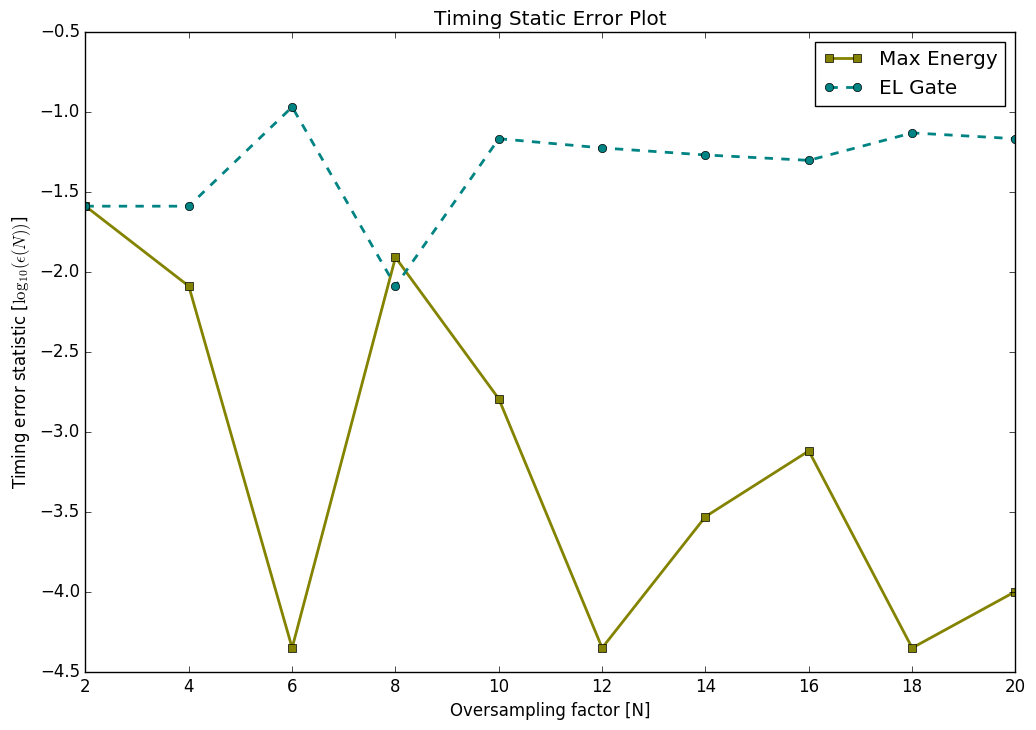
\includegraphics[width=.9\textwidth]{img/Timing-Static-Error}
\captionof{figure}{Timing Static Error vs RX Oversampling factor}
\label{err_stat}
\end{center}

As we can see on the figure \ref{err_stat}, the direct maximization of the output energy (Max Energy) is better than the indirect maximization (EL Gate). We can see both the direct and indirect maximization have an oscillation behavior.

\section{Lab Experiment}
\subsection{What is the symbol rate of the system based on the parameters above?}
The symbol rate of the system is 1 Mega symbol per second.
\subsection{Describe how the relationship between sampling error and oversample factor N manifests itself on the signal constellation}

\subsection{For each of the oversample factors in the previous question, specify what value you set the RX sample rate}
















































\end{document}
